\documentclass[12pt,fleqn]{article}
\usepackage[T1]{fontenc}
\usepackage{xiiiemc}
\usepackage{natbib}
%\usepackage{fancyhdr}
\usepackage{fancyhdr, graphicx}
\usepackage{fancyvrb}
\usepackage[os=win]{menukeys}       % Keyboard keys font (PC style)
\usepackage{color}
\usepackage{wallpaper}
\usepackage{titlesec}   %% Define space between paragraph e section
\usepackage{float} 	%% Use to fix Figure or Table: ex: \begin{table}[H]
%%%%Don't edit this block. It reduces the spacing between the lines of the
%%%%references
\let\OLDthebibliography\thebibliography
\renewcommand\thebibliography[1]{\OLDthebibliography{#1}
\setlength{\parskip}{0pt}\setlength{\itemsep}{0pt plus 0.3ex}}

%%-----------------------------------------------EDIT-----------------------------------------------
\title{Computabilidade --- Trabalho 1}

%%-----------------------------------------------EDIT----------------------------------------------
\author
    {\rm \begin{tabular}{l}
    \textbf{Ariel Nogueira Kovaljski}$^{1}$ - {\textnormal
    arielnogueirak@gmail.com}\\%
    {\fontsize{11}{0}\selectfont $^{1}$Universidade do Estado do Rio de
    Janeiro, Instituto Politécnico - Nova Friburgo, RJ,
    Brazil}\vspace*{-0.05cm} \\
  \end{tabular}}
%%----------------------------------------------------------------------------------------------
\fancypagestyle{firspagetstyle}
{

	\renewcommand{\headrulewidth}{0.0pt}
	\fancyfoot[C]{\footnotesize \parbox{15cm} {\centering
\fontsize{7.5}{0}\selectfont \it  }} % \ttfamil
	%\rhead{}
}



%%------------------

\begin{document}

\pretolerance10000
%\begin{figure}   % esse comando é para inserir a figura da logo da revista
%\centering
%
%\begin{minipage}[c]{\textwidth}
%\centering
%    
\includegraphics[width=5.75in]{logo.jpg}
%\end{minipage}
%\end{figure}

\vspace{-3cm}

\maketitle


\pagestyle{empty}

\thispagestyle{firspagetstyle}

\begin{abstract}
    Este trabalho trata-se sobre a definição de programas monolíticos,
    iterativos e recursivos; além disso, trata sobre a implementação de máquinas
    Norma e de Turing.
\end{abstract}

\keywords{\em{Programa Monolítico, Programa Iterativo, Programa Recursivo,
Máquina Norma, Máquina de Turing}}


%---------------------------------------------------------
\fancyhead[L]{\footnotesize{\fontsize{7.5}{0}\selectfont \it}}

\renewcommand{\headrulewidth}{0.0pt}
\fancyfoot[C]{\footnotesize \parbox{15cm} {\centering
\fontsize{7.5}{0}\selectfont \it  }} % \ttfamil
\rhead{}
%---------------------------------------------------------


\pagestyle{fancy}


\section{INTRODUÇÃO}
Em um mundo cada vez mais tecnológico, se faz cada vez mais necessário saber
sobre a teoria por trás do funcionamento da maior parte dos dispositivos do
nosso cotidiano. O conceito e diferentes definições de programa, assim como o
conhecimento sobre máquinas Norma e de Turing nos permite melhor apreciar e
aproveitar destas tecnologias, e conceber novos cenários onde a aplicação da
computabilidade pode vir a ser vantajosa.

\section{DESENVOLVIMENTO}

\subsection{Definição Formal de Programas}
Um conjunto estruturado de instruções que permitem uma máquina a realização
de operações e testes sobre dados de entrada, produzindo dados de saída, pode
ser definido como um programa.

Todo programa necessita de uma estrutura de controle de operações e testes, que
permite a composição destes segundo um conjunto de regras. Dentre as linguagens
de programação atuais, os tipos de estruturação mais comuns são: monolítica,
iterativa e recursiva.

\subsubsection{Programa Monolítico}
É definido como um tipo de programa onde sua estrutura é dada apenas por
desvios condicionais e incondicionais. A sua lógica, portanto, é distribuída
por um grande bloco (monólito) que constitui o programa.

A definição formal de um programa monolítico depende dos seguintes conceitos:

\begin{enumerate}
    \item rótulo/etiqueta: palavra sobre o alfabeto de letras ou dígitos;
    \item instrução rotulada/etiquetada: cadeia de caracteres da seguinte forma
        \subitem operação --- \texttt{$r_1$: faça <$F$ | \checkmark>
        vá\_para
        $r_2$}
        \subitem \hspace{1.5em} teste --- \texttt{$r_1$: se $T$ então vá\_para
        $r_2$ senão vá\_para $r_3$}
\end{enumerate}

\noindent
Um programa monolítico $P$ é um par ordenado:
\[
    P = (I, r)
\]
onde,

\begin{enumerate}
    \item $I$: conjunto finito de instruções rotuladas, todas distintas;
    \item $r$: rótulo inicial; instrução inicial em $I$;
    \item rótulo final: caso seja referido por uma instrução de $I$, mas não
    pertença a $I$.
\end{enumerate}

É possível ilustrar um programa monolítico por meio de um fluxograma, onde cada
componente deste é representado por um bloco. Dentre os blocos disponíveis
temos o de \textit{partida}, \textit{parada}, \textit{operação} e
\textit{teste}. Um caso especial é o da operação vazia \checkmark, onde o
retângulo correspondente à operação pode ser omitido.

\begin{figure}[H]
    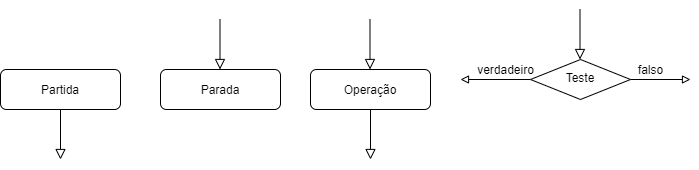
\includegraphics[width=\linewidth]{img/monolitico}
    \caption{Componentes de um programa monolítico em forma de fluxograma}
\end{figure}

\subsubsection{Exemplo de Programa Monolítico}
~
\begin{figure}[H]
\begin{verbatim}
    1: faça F vá_para 2
    2: se T1 então vá_para 1 senão vá_para 3
    3: faça G vá_para 4
    4: se T2 então vá_para 5 senão vá_para 1
\end{verbatim}
\caption{Exemplo de programa monolítico}
\end{figure}

\begin{figure}[H]
    \centering
    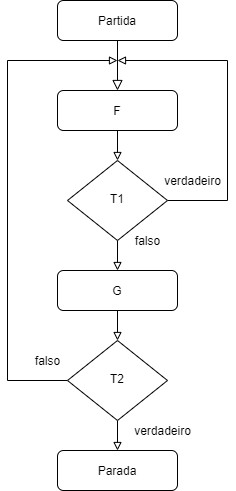
\includegraphics[height=10cm]{img/monolitico_ex}
    \caption{Exemplo de programa monolítico em forma de fluxograma}
\end{figure}

Para efeito de exemplo, considerando uma máquina de dois registradores, $(a,b)$,
as funções $F := (a := a+1) \rightarrow$ \verb|incrementa_a| e $G := (b := b-1)
\rightarrow$ \verb|decrementa_b|, os testes $T_1 := (a == 10)$ e $T_2 := (b ==
0)$ temos a seguinte máquina:

\begin{figure}[H]
\begin{verbatim}
    1: faça incrementa_a vá_para 2
    2: se (a == 10) então vá_para 1 senão vá_para 3
    3: faça decrementa_b vá_para 4
    4: se (b == 0) então vá_para 5 senão vá_para 1
\end{verbatim}
\caption{Exemplo de programa monolítico com funções e testes especificados}
\end{figure}

\noindent
Para um valor inicial de memória \verb|(5,2)|, a computação deste programa se dá
através dos seguintes passos:

\begin{figure}[H]
\begin{Verbatim}[commandchars=\\\{\},codes={\catcode`\$=3\catcode`\^=7}]
    (1,(5,3)) $\rightarrow$ instrução inicial e valor inicial armazenado
    (2,(6,2)) $\rightarrow$ em 1 $a$ é incrementado
    (3,(6,2)) $\rightarrow$ em 2 como $a \neq 10$, desviou para 3
    (4,(6,1)) $\rightarrow$ em 3 $b$ é decrementado
    (1,(7,1)) $\rightarrow$ em 4 como $b \neq 0$, desviou para 1
    (2,(7,1)) $\rightarrow$ em 1 $a$ é incrementado
    (3,(7,1)) $\rightarrow$ em 2 como $a \neq 10$, desviou para 3
    (4,(7,0)) $\rightarrow$ em 3 $b$ é decrementado
    (5,(7,0)) $\rightarrow$ em 4 como $b = 0$, desviou para 5. FIM.
\end{Verbatim}
\caption{Execução do programa monolítico para a entrada \texttt{(5,2)}}
\end{figure}


\subsubsection{Programa Iterativo}
Um programa iterativo pode ser considerado uma evolução de um programa
monolítico, devido a introdução de estruturas de controle que permitem um
melhor entendimento por trás da lógica e funcionalidade do programa. Através
das estruturas de controle iterativas, evitam-se os desvios incondicionais ---
os quais tem potencial para grandes ``quebras de lógica'', como o infamo
\verb|goto| --- substituindo-os por laços de repetição. Esta prática deu origem
ao conceito de programação estruturada, a qual é utilizada pela maioria das
linguagens de programação atuais.

É possível descrever a composição de um programa iterativo como a composição de
outros programas iterativos. Sendo assim, definem-se componentes básicos aos
mesmos:

\begin{enumerate}
    \item Operação vazia \checkmark;
    \item Identificadores de operação;
    \item Composição sequencial --- \texttt{$V$;$W$}: para programas iterativos
    $V$ e $W$, esta composição resulta na execução de $V$ e, em seguida,
    execução de $W$;
    \item Composição condicional --- \texttt{(se $T$ então $V$ senão $W$)}:
    Dado uma condição de teste $T$, a composição condicional executa $V$ se $T$
    é verdadeiro ou $W$ se $T$ é falso.
    \item Composição enquanto --- \texttt{enquanto $T$ faça  ($V$)}: resulta na
    execução repetida de $V$ enquanto a condição de teste $T$ for verdadeira;
    \item Composição até --- \texttt{até $T$ faça ($V$)}: funciona de maneira
    oposta à composição enquanto; executa $V$ repetidamente enquanto $T$ for
    falso.
\end{enumerate}

\subsubsection{Exemplo de Programa Iterativo}
~
\begin{figure}[H]
\begin{Verbatim}[commandchars=\\\{\},codes={\catcode`\$=3\catcode`\^=7}]
    se T1 então (enquanto T2 faça (até T3 faça (V;W))) senão \checkmark
\end{Verbatim}
\caption{Exemplo de programa iterativo}
\end{figure}

\begin{figure}[H]
    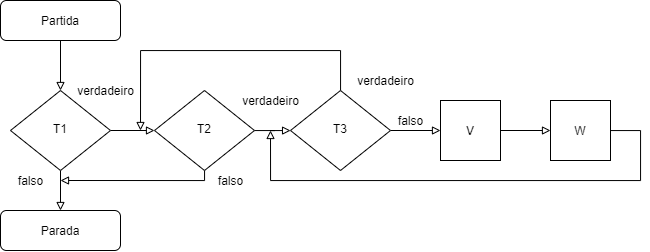
\includegraphics[width=\linewidth]{img/iterativo_ex}
    \caption{Exemplo de programa iterativo em forma de fluxograma}
\end{figure}

Para efeito de exemplo, considerando uma máquina de dois registradores, $(a,b)$,
as funções $V := (a := a-1) \rightarrow$ \verb|decrementa_a| e $W := (b := b+1)
\rightarrow$ \verb|incrementa_b|, os testes $T_1 := (a == 10)$, $T_2 := (a >
b)$, $T_3 := (b == 10)$ temos a seguinte máquina:

\begin{figure}[H]
\begin{Verbatim}[commandchars=\\\{\},codes={\catcode`\$=3\catcode`\^=7}]
    se (a == 10) então (
        enquanto (a > b) faça (
            até (b == 10) faça (
                decrementa_a;incrementa_b
            )
        )
    ) senão \checkmark
\end{Verbatim}
\caption{Exemplo de programa iterativo com funções e testes especificados}
\end{figure}

\noindent
Para um valor inicial de memória \verb|(10,2)|, a computação deste programa se
dá através dos seguintes passos:

\begin{figure}[H]
\begin{Verbatim}[commandchars=\\\{\},codes={\catcode`\$=3\catcode`\^=7}]
    MEMÓRIA | INSTRUÇÃO
    (10, 2) | se (a == 10) então    $\rightarrow$ 10 == 10 $\rightarrow$ verdadeiro
    (10, 2) | enquanto (a > b) faça $\rightarrow$ 10  >  2 $\rightarrow$ verdadeiro
    (10, 2) | até (b == 10) faça    $\rightarrow$  2 == 10 $\rightarrow$ falso
    (10, 2) | decrementa_a
    ( 9, 2) | incrementa_b
    ( 9, 3) | até (b == 10) faça    $\rightarrow$  3 == 10 $\rightarrow$ falso
    ( 9, 3) | decrementa_a
    ( 8, 3) | incrementa_b
    ( 8, 4) | até (b == 10) faça    $\rightarrow$  4 == 10 $\rightarrow$ falso
    ( 8, 4) | decrementa_a
    ( 7, 4) | incrementa_b
    ( 7, 5) | até (b == 10) faça    $\rightarrow$  5 == 10 $\rightarrow$ falso
    ( 7, 5) | decrementa_a
    ( 6, 5) | incrementa_b
    ( 6, 6) | até (b == 10) faça    $\rightarrow$  6 == 10 $\rightarrow$ falso
    ( 6, 6) | decrementa_a
    ( 5, 6) | incrementa_b
    ( 5, 7) | até (b == 10) faça    $\rightarrow$  7 == 10 $\rightarrow$ falso
    ( 5, 7) | decrementa_a
    ( 4, 7) | incrementa_b
    ( 4, 8) | até (b == 10) faça    $\rightarrow$  8 == 10 $\rightarrow$ falso
    ( 4, 8) | decrementa_a
    ( 3, 8) | incrementa_b
    ( 3, 9) | até (b == 10) faça    $\rightarrow$  9 == 10 $\rightarrow$ falso
    ( 3, 9) | decrementa_a
    ( 2, 9) | incrementa_b
    ( 2,10) | até (b == 10) faça    $\rightarrow$ 10 == 10 $\rightarrow$ verdadeiro
    ( 2,10) | enquanto (a > b)      $\rightarrow$  2  > 10 $\rightarrow$ falso
    ( 2,10) | \checkmark FIM
\end{Verbatim}
\caption{Execução do programa iterativo para a entrada \texttt{(10,2)}}
\end{figure}

\subsubsection{Programa Recursivo}
Também encontrado na maior parte das linguagens de programação atuais, é um
tipo de estrutura onde uma rotina é composta por sub-rotinas que são compostas
de chamadas à rotina original. Desta forma, a execução de um programa recursivo
pode ser expandida em camadas, onde sucessivas chamadas à rotina em níveis cada
vez mais profundos levam a um resultado que, no fim da recursão, é
retro-propagado até a rotina de superfície.

Sub-rotinas podem ser definidas como expressões. Os seguintes itens
caracterizam-se como expressões de sub-rotinas:

\begin{enumerate}
    \item Operação vazia \checkmark;
    \item Identificadores de operação;
    \item Identificadores de sub-rotina;
    \item Composição sequencial --- \texttt{($D_1$;$D_2$)}: Para $D_1$ e $D_2$
    expressões de sub-rotinas, a sua composição sequencial resulta na execução
    de $D_1$ e, em seguida, execução de $D_2$;
    \item Composição condicional --- \texttt{(se $T$ então $D_1$ senão $D_2$)}:
    Dado um condição de teste $T$, a composição condicional é uma expressão de
    sub-rotinas que executa $D_1$ se $T$ é verdadeiro ou $D_2$ se $T$ é falso.
\end{enumerate}

Um programa recursivo $P$, portanto, pode ser definido por uma composição de
expressões de sub-rotinas, de forma que:
\[
    P \text{\tt\ é\ } E_0 \text{\tt\ onde\ } R_1 \text{\tt\ def\ } E_1, R_2
    \text{\tt\ def\ } E_2, \dots, R_n \text{\tt\ def\ } E_n
\]

Para cada $E_k, k \in \{1, 2, \dots, n\}$, temos:

\begin{itemize}
    \item $E_0$: Expressão inicial;
    \item $E_k$: Expressão que define a sub-rotina $R_k$;
\end{itemize}

\subsubsection{Exemplo de Programa Recursivo}
~
\begin{figure}[H]
\begin{Verbatim}[commandchars=\\\{\},codes={\catcode`\$=3\catcode`\^=7}]
    R def (se T1 então G senão S;R),
    S def H;I
\end{Verbatim}
\caption{Exemplo de programa recursivo}
\end{figure}

Para efeito de exemplo, considerando uma máquina de dois registradores, $(a,b)$,
as funções $G := (\checkmark)$, $H := (a := a-1) \rightarrow$
\verb|decrementa_a| e $I := (b := b+1) \rightarrow$ \verb|incrementa_b|, os
testes $T_1 := (a == 0)$, temos a seguinte máquina:

\begin{figure}[H]
\begin{Verbatim}[commandchars=\\\{\},codes={\catcode`\$=3\catcode`\^=7}]
    R def (se (a == 0) então \checkmark senão S;R),
    S def decrementa_a;incrementa_b
\end{Verbatim}
\caption{Exemplo de programa recursivo com funções e testes especificados}
\end{figure}

\noindent
Para um valor inicial de memória \verb|(5,0)|, a computação deste programa se
dá através dos seguintes passos:

\begin{figure}[H]
\begin{Verbatim}[commandchars=\\\{\},codes={\catcode`\$=3\catcode`\^=7}]
    (R; \checkmark,5,0)

    (se (a == 0) então \checkmark senão (S;R); \checkmark,5,0)
    (S;R; \checkmark,5,0)
    (decrementa_a;incrementa_b;R; \checkmark,5,0)
    (incrementa_b;R; \checkmark,4,0)
    (R; \checkmark,4,1)

    (se (a == 0) então \checkmark senão (S;R); \checkmark,4,1)
    (S;R; \checkmark,4,1)
    (decrementa_a;incrementa_b;R; \checkmark,4,1)
    (incrementa_b;R; \checkmark,3,1)
    (R; \checkmark,3,2)

    (se (a == 0) então \checkmark senão (S;R); \checkmark,3,2)
    (S;R; \checkmark,3,2)
    (decrementa_a;incrementa_b;R; \checkmark,3,2)
    (incrementa_b;R; \checkmark,2,2)
    (R; \checkmark,2,3)

    (se (a == 0) então \checkmark senão (S;R); \checkmark,2,3)
    (S;R; \checkmark,2,3)
    (decrementa_a;incrementa_b;R; \checkmark,2,3)
    (incrementa_b;R; \checkmark,1,3)
    (R; \checkmark,1,4)

    (se (a == 0) então \checkmark senão (S;R); \checkmark,1,4)
    (S;R; \checkmark,1,4)
    (decrementa_a;incrementa_b;R; \checkmark,1,4)
    (incrementa_b;R; \checkmark,0,4)
    (R; \checkmark,0,5)

    (se (a == 0) então \checkmark senão (S;R); \checkmark,0,5)
    (\checkmark; \checkmark,0,5)
    (\checkmark,0,5)
\end{Verbatim}
\caption{Execução do programa recursivo para a entrada \texttt{(5,0)}}
\end{figure}

\newpage
\subsection{Tradução de Fluxogramas para Programas Monolíticos e Recursivos}

\subsubsection{Diagrama (a)}
~
\begin{figure}[H]
    \centering
    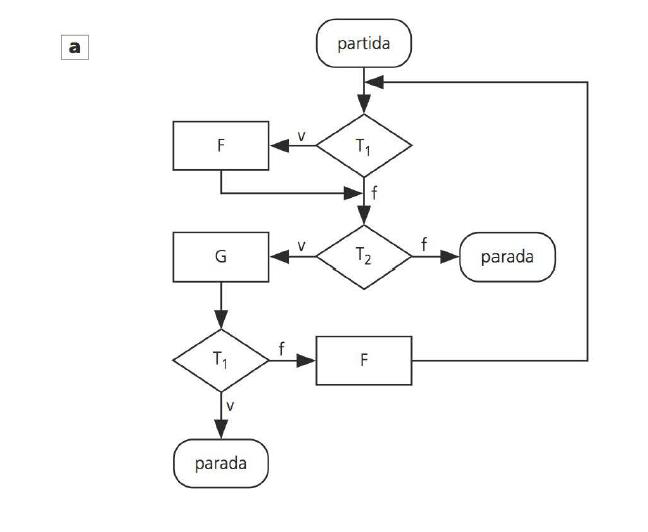
\includegraphics[height=7.5cm]{img/diagrama_a}
\end{figure}
%
\begin{figure}[H]
\begin{verbatim}
    1: se T1 vá_para 2 senão vá_para 3
    2: faça F vá_para 3
    3: se T2 vá_para 4 senão vá_para 7
    4: faça G vá_para 5
    5: se T1 vá_para 7 senão vá_para 6
    6: faça F vá_para 1
\end{verbatim}
\caption{Tradução do fluxograma (a) para um programa monolítico}
\end{figure}
%
\begin{figure}[H]
\begin{Verbatim}[commandchars=\\\{\},codes={\catcode`\$=3\catcode`\^=7}]
    P é R1 onde
        R1 def (se T1 então R2 senão R3),
        R2 def (F;R3),
        R3 def (se T2 então R4 senão R7),
        R4 def (G;R5),
        R5 def (se T1 então R7 senão R6),
        R6 def (F;R1)
        R7 def \checkmark
\end{Verbatim}
\caption{Tradução do fluxograma (a) para um programa recursivo}
\end{figure}

\newpage
\subsubsection{Diagrama (b)}
~
\begin{figure}[H]
    \centering
    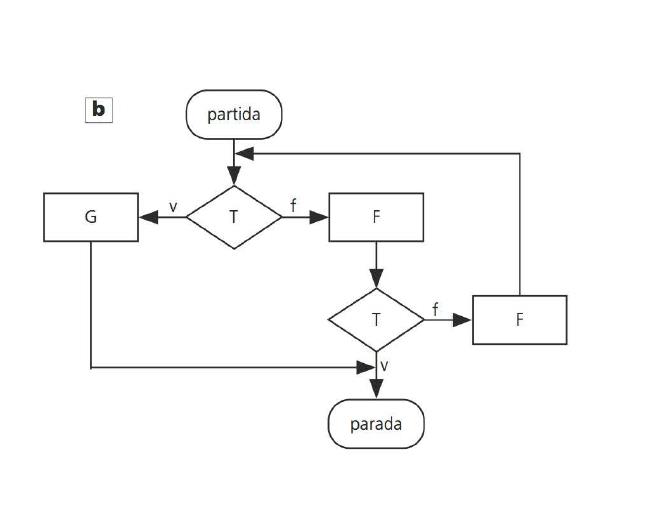
\includegraphics[height=7.5cm]{img/diagrama_b}
\end{figure}
%
\begin{figure}[H]
\begin{verbatim}
    1: se T faça vá_para 2 senão vá_para 3
    2: faça G vá_para 6
    3: faça F vá_para 4
    4: se T faça vá_para 6 senão vá_para 5
    5: faça F vá_para 1
\end{verbatim}
\caption{Tradução do fluxograma (b) para um programa monolítico}
\end{figure}
%
\begin{figure}[H]
\begin{Verbatim}[commandchars=\\\{\},codes={\catcode`\$=3\catcode`\^=7}]
    P é R1 onde
        R1 def (se T então R2 senão R3),
        R2 def (G;R6),
        R3 def (F;R4),
        R4 def (se T então R6 senão R5),
        R5 def (F;R1),
        R6 def \checkmark
\end{Verbatim}
\caption{Tradução do fluxograma (b) para um programa recursivo}
\end{figure}

\newpage
\subsubsection{Diagrama (c)}
~
\begin{figure}[H]
    \centering
    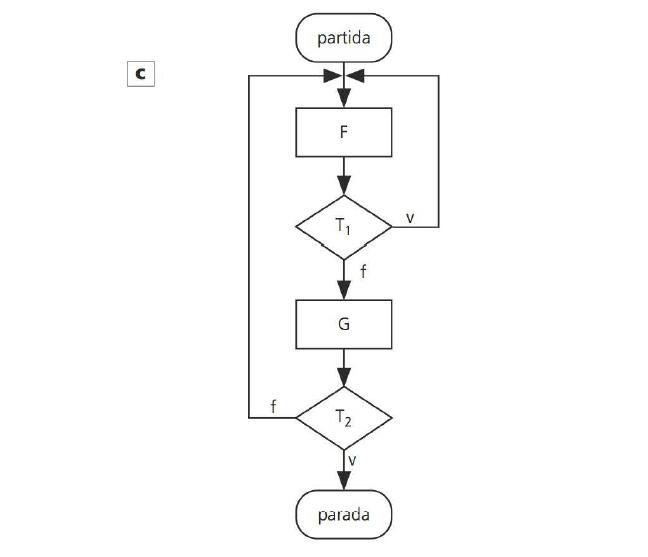
\includegraphics[height=7.5cm]{img/diagrama_c}
\end{figure}
%
\begin{figure}[H]
\begin{verbatim}
    1: faça F vá_para 2
    2: se T1 vá_para 1 senão vá_para 3
    3: faça G vá_para 4
    4: se T2 vá_para 5 senão vá_para 1
\end{verbatim}
\caption{Tradução do fluxograma (c) para um programa monolítico}
\end{figure}
%
\begin{figure}[H]
\begin{Verbatim}[commandchars=\\\{\},codes={\catcode`\$=3\catcode`\^=7}]
    P é R1 onde
        R1 def (F;R2),
        R2 def (se T1 então R1 senão R3),
        R3 def (G;R4),
        R4 def (se T2 então R5 senão R1),
        R5 def \checkmark
\end{Verbatim}
\caption{Tradução do fluxograma (c) para um programa recursivo}
\end{figure}

\newpage
\subsubsection{Diagrama (d)}
~
\begin{figure}[H]
    \centering
    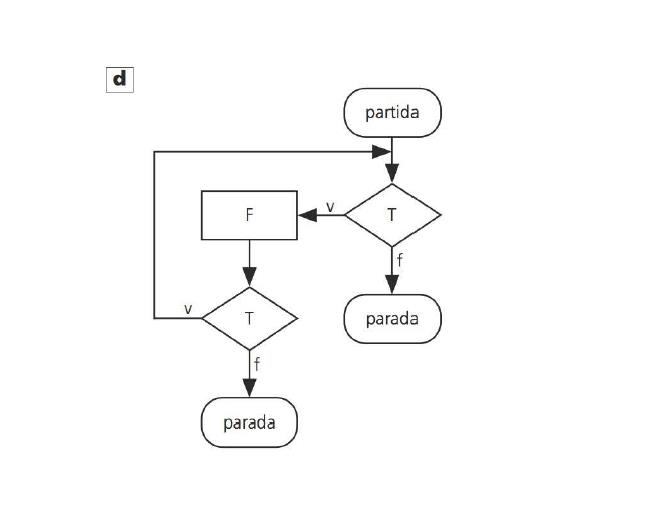
\includegraphics[height=7.5cm]{img/diagrama_d}
\end{figure}
%
\begin{figure}[H]
\begin{verbatim}
    1: se T vá_para 2 senão vá_para 4
    2: faça F vá_para 3
    3: se T vá_para 1 senão vá_para 4
\end{verbatim}
\caption{Tradução do fluxograma (d) para um programa monolítico}
\end{figure}
%
\begin{figure}[H]
\begin{Verbatim}[commandchars=\\\{\},codes={\catcode`\$=3\catcode`\^=7}]
    P é R1 onde
        R1 def (se T então R2 senão R4)
        R2 def (F;R3)
        R3 def (se T então R1 senão R4)
        R4 def \checkmark
\end{Verbatim}
\caption{Tradução do fluxograma (d) para um programa recursivo}
\end{figure}

\subsection{Implementação de uma Máquina Norma}
<INSERIR TEXTO SOBRE MÁQUINA NORMA>

\subsection{Implementação de uma Máquina de Turing}
A implementação da máquina de Turing (MT) foi realizada através da linguagem de
programação \textit{Python}, pois sua orientação a objetos e simplicidade de
sintaxe permitiu uma modelagem do problema de forma mais direta, rápida e
eficiente.

A mesma consiste de duas classes: uma para a lógica do programa
(\verb|TuringMachine|), e a outra para a fita (\verb|Tape|).

Na classe \verb|TuringMachine|, as quíntuplas da MT, são armazenadas em um
dicionário, onde cada elemento do dicionário corresponde a um estado, cada
estado é um dicionário que contém os símbolos de entrada, e cada símbolo de
entrada é um dicionário que contém a própria quíntupla, isto é, estado atual
(\verb|present_state|), símbolo de entrada (\verb|present_symbol|), símbolo de
saída (\verb|symbol_printed|), direção (\verb|direction|) e o próximo estado
(\verb|next_state|).

<INSERIR FIGURA - LÓGICA DE FUNCIONAMENTO DA MÁQUINA DE TURING>

A essência do funcionamento da MT é apresentada na figura acima, onde, para um
dado estado, dependendo do símbolo de \textit{input}, pode-se ter diferentes
símbolos de \textit{output}, direções e próximos estados.

Na classe \verb|Tape|, a fita é implementada como uma lista de comprimento
flexível, grande o suficiente para armazenar os dados com algumas células em
branco ao redor, que será preenchida com a \textit{string} de entrada.

Tanto o dicionário de quíntuplas quanto os dados de entrada da fita são
preenchidos a partir da leitura de um arquivo \verb|.yaml|, onde o usuário pode
configurar os parâmetros da MT.

Ao iniciar o programa, o mesmo realiza a inicialização de instâncias da MT e da
fita, e exibe no console uma mensagem de confirmação: caso o usuário pressione
\keys{\return}, a execução da MT é iniciada, caso o usuário pressione
\keys{\ctrl+C} ou \keys{\ctrl+D}, o programa é encerrado. Partindo do
pressuposto que o usuário decidiu iniciar a execução, o programa irá mostrar no
console uma representação visual da fita, os dados nela presentes, e do cabeçote
de leitura e escrita.

<INSERIR FIGURA - EXECUÇÃO DA MÁQUINA DE TURING>

Os seguintes elementos podem ser vistos nesta imagem:

\begin{enumerate}
    \item Iteração atual;
    \item Ação atual do cabeçote (Leitura (\verb|R|) ou Escrita (\verb|W|));
    \item Fita e seu conteúdo;
    \item Posição atual do cabeçote (representado pelo par \verb|> <|).
\end{enumerate}

A cada iteração o cabeçote realiza uma etapa de leitura e uma etapa de escrita.
Durante a leitura, o símbolo lido é comparado com os símbolos de \textit{input}
para aquele estado. Em seguida, o símbolo de \textit{output} é escrito, a MT
assume o novo estado, e o cabeçote se move em uma nova direção. Caso o próximo
estado não exista, ou o símbolo de entrada não conste dentre os \textit{inputs}
do estado atual, o programa encerrará a sua execução.

Devido a impossibilidade de se determinar para quais conjuntos de entradas e
quíntuplas a MT irá concluir sua execução ou ficará em um \textit{loop} infinito
(Halting Problem), é possível estabelecer um número máximo de iterações para a
MT através de um parâmetro no arquivo \verb|.yaml|. Caso o usuário deseje, este
também pode parar a execução do programa a qualquer momento, pressionando
\keys{\ctrl+C}.

Devido aos limites físicos de um computador real em relação à MT teórica --- no
caso, memória finita --- caso o cabeçote passe dos limites da fita, a execução
do programa será encerrada.

\subsubsection{Resultados}
Realizou-se a configuração da MT para o reconhecimento de duas linguagens
distintas, as quais serão apresentadas abaixo.

\subsubsection{Linguagem A}
Esta foi definida segundo a seguinte expressão regular: \verb|gggh*|.
Isto é, a mesma gera um conjunto de palavras que começa com \verb|ggg| e então é
seguindo de zero ou mais \verb|h|.

<INSERIR FIGURA - RESULTADO POSITIVO OPERAÇÃO MÁQUINA DE TURING LINGUAGEM A>

Como pode ser visto pela figura acima, a máquina aceita corretamente a entrada
\verb|ggghhhhhhhhh|, a qual pertence à linguagem A.

<INSERIR FIGURA - RESULTADO NEGATIVO OPERAÇÃO MÁQUINA DE TURING LINGUAGEM A>

Já nesta outra figura, vemos que a entrada \verb|gghhhhhhhhh| não é aceita pela
máquina, uma vez que a mesma não pertence à linguagem A.

\subsubsection{Linguagem B}
Esta foi definida segundo a seguinte expressão regular:
\verb|g*(hhh)+g|. Isto é, a mesma gera um conjunto de palavras que começa com
zero ou mais \verb|g|, o qual é necessariamente seguido por uma ou mais triplas
\verb|hhh| e termina com um único \verb|g|.

<INSERIR FIGURA - RESULTADO POSITIVO OPERAÇÃO MÁQUINA DE TURING LINGUAGEM B>

Como pode ser visto pela figura acima, a máquina aceita corretamente a entrada
\verb|ggggghhhhhhg|, a qual pertence à linguagem B.

<INSERIR FIGURA - RESULTADO NEGATIVO OPERAÇÃO MÁQUINA DE TURING LINGUAGEM B>

Já nesta outra figura, vemos que a entrada \verb|ghhhhhg| não é aceita pela
máquina, uma vez que a mesma não pertence à linguagem B.

\subsection{Uso das Máquinas de Turing}
Devido a presença de uma CPU, instruções programadas, um fluxo de entrada e de
saída de dados, essencialmente todos os dispositivos eletrônicos modernos podem
ser considerados máquinas de Turing. Isto inclui celulares, computadores,
tablets, consoles de vídeo-game e outros aparelhos conhecidos; mas também inclui
alguns dispositivos inesperados, como televisões, lâmpadas inteligentes, robôs
aspiradores, carros, cartões de crédito, escovas de dentes inteligentes, dentre
muitos outros. Em um mundo cada vez mais conectado, com a expansão da Internet
das Coisas (IoT) e da Nuvem, cada vez mais dispositivos irão contar com algum
poder computacional e portanto poderão ser considerados máquinas de Turing.

Existe, porém, uma tecnicalidade que é importante mencionar: as máquinas de
Turing são um conceito teórico. Devido a sua capacidade de memória infinita, não
é possível construir uma na realidade. Apesar disso, os computadores atuais são
o modelo mais próximo da mesma, exceto pela quantidade de memória finita. O que
isso significa na prática? Há certos problemas que não são computáveis em
computadores atuais devido a limitações de memória, mas que poderiam ser
resolvidas em uma máquina de Turing, dado tempo o suficiente. A classe de
problemas solucionáveis por computadores, porém, aumenta conforme os avanços
tecnológicos permitem \textit{hardware} cada vez mais potente e maior capacidade
de memória.

\newpage
\section{CONCLUSÕES}
Neste trabalho foi possível aprender a teoria e funcionamento por trás de
máquinas de Turing e máquinas Norma, ambas pertencentes a classe de máquinas
universais, e portanto, equivalentes em poder computacional. O uso destas para o
processamento de dados é indispensável nos dias atuais, e, com o avanço
tecnológico, cada vez mais aparelhos e objetos terão algum poder de
processamento, como é o caso da Internet das Coisas (IoT). Isso significa que a
computabilidade e suas teorias e aplicações estão sempre presentes em nosso
entorno, e passarão a contar com um papel cada vez mais fundamental em nossas
vidas.

% ------------------------------------------------------------------------
\begin{thebibliography}{99}
\fontsize{11}{0}\selectfont
\bibitem[Devirio, 2011]{Diverio11}
Diverio, T. A., Menezes, P. B. (2011). Teoria da Computação: Máquinas Universais
e Computabilidade - Vol.5. Brazil: Bookman.
\end{thebibliography}
\vspace*{-0.1cm}
\section*{APPENDIX A}
% ------------------------------------------------------------------------

%For papers written in Portuguese or Spanish.

\begin{center}
  Computability --- First Assignment
\end{center}

\def\abstractname{Abstract}%

\begin{abstract}
   This assignment discusses about the definition of monolithic, iterative and
   recursive programs; it also touches on the implementation of Norma and
   Turing Machines.
\end{abstract}

\keywords{\em{
    Monolithic Program, Iterative Program, Recursive Program,
    Norma Machine, Turing Machine
}}

\end{document}
